\chapter{Description of [APPNAME]}
\label{chp:description}

This chapter will give a description of [APPNAME], through textual description and screen shots.

\section{Basic System Architecture}
Figure \ref{fig:basic-architecture} shows an overview of the architecture we intend to use for our solution. We will build upon the architecture used by Aaberg et. al. \cite{CustomerDriven}.

We have access to a MySQL-server hosted at NTNU, which we will access by a PHP-server hosted at NTNU. The main reason we have to access the database through a server layer, is that it is quite cumbersome to connect to the database if a device is not connected at NTNU's network. In addition, by having a webservice do some of the work for us, it becomes easier to parse results from the database through JSON.   


The downside by having this approach is that scalability suffers from this architectural choice. However, we consider these problems as outside the scope of our thesis, and will continue using this approach.

\begin{figure}
		\centering
			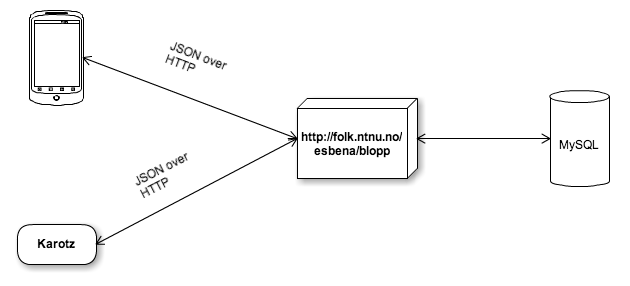
\includegraphics[width=0.50\paperwidth]{Pictures/basic-architecture.png}
		\caption{Basic architecture of our system}
		\label{fig:basic-architecture}
\end{figure}


\section{Child partition}
The child partition of our application consists mainly out of four parts. 

\paragraph{Treatment}
Figure \ref{fig:capp_start_treatment} shows a screenshot for the application when the child starts their medication. Starting this sequence can come from one out of two events: (i) \emph{The child reacts to an alarm set in the guardian partition}, and (ii) \emph{The child needs to take their medicine by need}. If (ii) is the case, the child is instructed to pick the medicine from a list shown by the application. If (i) is the case, the medicine is chosen beforehand. When a child has started their treatment, they are taken through an animated sequence, which reacts when a child interacts with the device.  


\begin{figure}
		\centering
			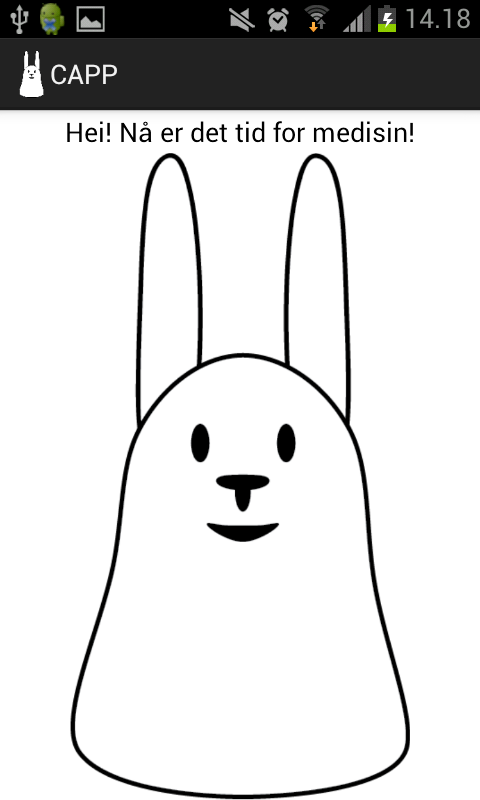
\includegraphics[width=0.50\paperwidth]{Pictures/app-screenshots/capp_start_treatment.png}
		\caption{Starting a treatment}
		\label{fig:capp_start_treatment}
\end{figure}

\paragraph{Show credits}

Figure \ref{fig:capp_stars} shows a screenshot for the application when the child wants to review how many stars he/she has received, based on the amount of medicine they have taken. 
\begin{figure}
		\centering
			
\includegraphics[width=0.50\paperwidth]{Pictures/app-screenshots/capp_stars.png}
		\caption{Stars}
		\label{fig:capp_stars}
\end{figure}


\paragraph{Shop}

\paragraph{Treatment instructions}

\section{Guardian partition}



% Basic arkitektur
% Skjermbilder -> Forklaringer
% Dropper alt som har med Karotz å gjøre, med unntak av ``konsept''-følelsen
% 